% Delta Lake Advanced - Comprehensive Notes
% LaTeX Beamer Presentation with Databricks Theme
% Generated for Day 5 of Databricks 14-Days AI Challenge

\documentclass[aspectratio=169]{beamer}

% ============================================
% PACKAGES
% ============================================
\usepackage{tikz}
\usepackage{graphicx}
\usepackage{hyperref}
\usepackage{xcolor}
\usepackage{listings}
\usepackage{fontawesome5}
\usepackage{booktabs}
\usepackage{array}
\usepackage{colortbl}
\usepackage{multirow}
\usepackage{amsmath}

% ============================================
% DATABRICKS COLOR PALETTE
% ============================================
\definecolor{databricksBlue}{RGB}{41, 49, 66}
\definecolor{databricksRed}{RGB}{220, 53, 69}
\definecolor{databricksYellow}{RGB}{255, 193, 7}
\definecolor{databricksGreen}{RGB}{76, 175, 80}
\definecolor{databricksGray}{RGB}{128, 128, 128}
\definecolor{databricksLightGray}{RGB}{245, 245, 245}
\definecolor{databricksWhite}{RGB}{255, 255, 255}
\definecolor{codeBackground}{RGB}{40, 44, 52}
\definecolor{codeText}{RGB}{171, 178, 191}
\definecolor{codeKeyword}{RGB}{198, 120, 221}
\definecolor{codeString}{RGB}{152, 195, 121}
\definecolor{codeComment}{RGB}{92, 99, 112}

% ============================================
% BEAMER THEME CONFIGURATION
% ============================================
\usetheme{default}
\setbeamercolor{background canvas}{bg=databricksWhite}
\setbeamercolor{normal text}{fg=databricksBlue}
\setbeamercolor{frametitle}{fg=databricksWhite,bg=databricksBlue}
\setbeamercolor{title}{fg=databricksWhite}
\setbeamercolor{subtitle}{fg=databricksLightGray}
\setbeamercolor{author}{fg=databricksWhite}
\setbeamercolor{institute}{fg=databricksLightGray}
\setbeamercolor{date}{fg=databricksLightGray}
\setbeamercolor{itemize item}{fg=databricksBlue}
\setbeamercolor{itemize subitem}{fg=databricksRed}
\setbeamercolor{block title}{fg=databricksWhite,bg=databricksBlue}
\setbeamercolor{block body}{bg=databricksLightGray}

\setbeamertemplate{itemize item}{\textcolor{databricksBlue}{$\bullet$}}
\setbeamertemplate{itemize subitem}{\textcolor{databricksRed}{$\triangleright$}}
\setbeamertemplate{navigation symbols}{}

% ============================================
% CODE LISTINGS STYLE
% ============================================
\lstdefinestyle{sqlstyle}{
    backgroundcolor=\color{codeBackground},
    basicstyle=\ttfamily\scriptsize\color{codeText},
    keywordstyle=\color{codeKeyword}\bfseries,
    stringstyle=\color{codeString},
    commentstyle=\color{codeComment}\itshape,
    breaklines=true,
    showstringspaces=false,
    frame=single,
    rulecolor=\color{databricksBlue},
    numbers=none,
    xleftmargin=3pt,
    xrightmargin=3pt,
    aboveskip=8pt,
    belowskip=5pt,
    morekeywords={SELECT, FROM, WHERE, INSERT, UPDATE, DELETE, MERGE, INTO, USING, ON, WHEN, MATCHED, NOT, THEN, SET, VALUES, AS, AND, OR, VERSION, OF, TIMESTAMP, DESCRIBE, HISTORY, RESTORE, TABLE, TO, OPTIMIZE, ZORDER, BY, VACUUM, RETAIN, HOURS, DRY, RUN, ALTER, TBLPROPERTIES, LIMIT, true, false}
}

\lstdefinestyle{pythonstyle}{
    backgroundcolor=\color{codeBackground},
    basicstyle=\ttfamily\scriptsize\color{codeText},
    keywordstyle=\color{codeKeyword}\bfseries,
    stringstyle=\color{codeString},
    commentstyle=\color{codeComment}\itshape,
    breaklines=true,
    showstringspaces=false,
    frame=single,
    rulecolor=\color{databricksBlue},
    numbers=none,
    xleftmargin=3pt,
    xrightmargin=3pt,
    aboveskip=8pt,
    belowskip=5pt,
    morekeywords={from, import, def, return, if, else, for, in, as, True, False, None, print, class, self}
}

% ============================================
% CUSTOM FOOTER
% ============================================
\setbeamertemplate{footline}{
    \leavevmode%
    \hbox{%
        \begin{beamercolorbox}[wd=.333333\paperwidth,ht=2.5ex,dp=1ex,left]{author in head/foot}%
            \usebeamerfont{author in head/foot}\hspace*{2ex}%
            \href{https://easy-ai-labs.lovable.app/}{\textcolor{databricksBlue}{\faRocket\ Easy AI Labs}}
        \end{beamercolorbox}%
        \begin{beamercolorbox}[wd=.333333\paperwidth,ht=2.5ex,dp=1ex,center]{title in head/foot}%
            \usebeamerfont{title in head/foot}%
            \href{https://www.linkedin.com/in/yashkavaiya}{\textcolor{databricksBlue}{\faLinkedin\ Yash Kavaiya}}
        \end{beamercolorbox}%
        \begin{beamercolorbox}[wd=.333333\paperwidth,ht=2.5ex,dp=1ex,right]{date in head/foot}%
            \usebeamerfont{date in head/foot}%
            \href{https://www.linkedin.com/company/genai-guru}{\textcolor{databricksBlue}{Gen AI Guru \faUsers}}\hspace*{2ex}
            \textcolor{databricksGray}{\insertframenumber{} / \inserttotalframenumber}\hspace*{2ex}
        \end{beamercolorbox}%
    }%
    \vskip0pt%
}

% ============================================
% TITLE PAGE TEMPLATE
% ============================================
\defbeamertemplate*{title page}{customized}[1][]
{
    \begin{tikzpicture}[remember picture,overlay]
        \fill[databricksBlue] (current page.north west) rectangle (current page.south east);
    \end{tikzpicture}
    \vfill
    \begin{center}
        {\Huge\textcolor{databricksWhite}{\textbf{\inserttitle}}\par}
        \vspace{0.5cm}
        {\Large\textcolor{databricksYellow}{\insertsubtitle}\par}
        \vspace{1cm}
        {\large\textcolor{databricksWhite}{\insertauthor}\par}
        \vspace{0.3cm}
        {\small\textcolor{databricksLightGray}{\insertinstitute}\par}
        \vspace{0.5cm}
        {\small\textcolor{databricksLightGray}{\insertdate}\par}
    \end{center}
    \vfill
}

% ============================================
% DOCUMENT METADATA
% ============================================
\title{Delta Lake Advanced}
\subtitle{Time Travel, MERGE, OPTIMIZE \& VACUUM}
\author{Databricks 14-Days AI Challenge}
\institute{Day 5 - Advanced Delta Lake Features}
\date{\today}

\begin{document}

% ============================================
% TITLE SLIDE
% ============================================
\begin{frame}[plain]
    \titlepage
\end{frame}

% ============================================
% TABLE OF CONTENTS
% ============================================
\begin{frame}[fragile]{Agenda}
    \begin{columns}[T]
        \begin{column}{0.48\textwidth}
            \begin{itemize}
                \item \textcolor{databricksBlue}{\textbf{Delta Lake Architecture}}
                    \begin{itemize}
                        \item Transaction Log \& Parquet Files
                        \item ACID Properties
                    \end{itemize}
                \item \textcolor{databricksBlue}{\textbf{Time Travel}}
                    \begin{itemize}
                        \item Version History Queries
                        \item Restore Operations
                    \end{itemize}
                \item \textcolor{databricksBlue}{\textbf{MERGE Operations}}
                    \begin{itemize}
                        \item Upsert Patterns
                        \item SCD Type 2
                    \end{itemize}
            \end{itemize}
        \end{column}
        \begin{column}{0.48\textwidth}
            \begin{itemize}
                \item \textcolor{databricksBlue}{\textbf{OPTIMIZE \& ZORDER}}
                    \begin{itemize}
                        \item File Compaction
                        \item Data Skipping
                    \end{itemize}
                \item \textcolor{databricksBlue}{\textbf{VACUUM for Cleanup}}
                    \begin{itemize}
                        \item Stale File Removal
                        \item Retention Configuration
                    \end{itemize}
                \item \textcolor{databricksBlue}{\textbf{Best Practices}}
                    \begin{itemize}
                        \item Performance Tips
                        \item Common Pitfalls
                    \end{itemize}
            \end{itemize}
        \end{column}
    \end{columns}
\end{frame}

% ============================================
% SECTION: Delta Lake Architecture
% ============================================
\begin{frame}[fragile]{Delta Lake Architecture Overview}
    \begin{columns}[T]
        \begin{column}{0.55\textwidth}
            \textcolor{databricksBlue}{\textbf{What is Delta Lake?}}\\[0.3cm]
            An open-source storage layer that brings \textbf{ACID transactions} to Apache Spark and big data workloads.
            
            \vspace{0.5cm}
            \textcolor{databricksBlue}{\textbf{Core Components:}}
            \begin{itemize}
                \item \textcolor{databricksRed}{$\triangleright$} \textbf{Transaction Log (\_delta\_log)}
                    \begin{itemize}
                        \item JSON files recording every change
                        \item Enables ACID \& time travel
                    \end{itemize}
                \item \textcolor{databricksRed}{$\triangleright$} \textbf{Parquet Data Files}
                    \begin{itemize}
                        \item Efficient columnar storage
                        \item Optimized compression
                    \end{itemize}
            \end{itemize}
        \end{column}
        \begin{column}{0.42\textwidth}
            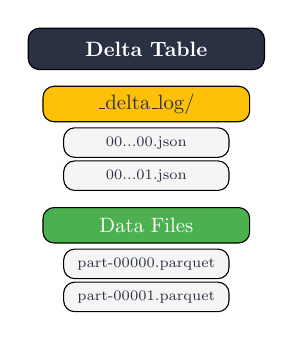
\begin{tikzpicture}[scale=0.7, every node/.style={scale=0.75}]
                \node[draw, fill=databricksBlue, text=white, rounded corners, minimum width=4cm, minimum height=0.7cm] at (0,4) {\textbf{Delta Table}};
                \node[draw, fill=databricksYellow, text=databricksBlue, rounded corners, minimum width=3.5cm, minimum height=0.6cm] at (0,3) {\_delta\_log/};
                \node[draw, fill=databricksLightGray, text=databricksBlue, rounded corners, minimum width=2.8cm, minimum height=0.5cm, font=\scriptsize] at (0,2.3) {00...00.json};
                \node[draw, fill=databricksLightGray, text=databricksBlue, rounded corners, minimum width=2.8cm, minimum height=0.5cm, font=\scriptsize] at (0,1.7) {00...01.json};
                \node[draw, fill=databricksGreen, text=white, rounded corners, minimum width=3.5cm, minimum height=0.6cm] at (0,0.8) {Data Files};
                \node[draw, fill=databricksLightGray, text=databricksBlue, rounded corners, minimum width=2.8cm, minimum height=0.5cm, font=\scriptsize] at (0,0.1) {part-00000.parquet};
                \node[draw, fill=databricksLightGray, text=databricksBlue, rounded corners, minimum width=2.8cm, minimum height=0.5cm, font=\scriptsize] at (0,-0.5) {part-00001.parquet};
            \end{tikzpicture}
        \end{column}
    \end{columns}
\end{frame}

% ============================================
% ACID Properties
% ============================================
\begin{frame}[fragile]{ACID Properties in Delta Lake}
    \begin{columns}[T]
        \begin{column}{0.48\textwidth}
            \textcolor{databricksBlue}{\Large\textbf{A}}\textbf{tomicity}\\[0.2cm]
            Each transaction completely succeeds or completely fails. Partial changes are never visible.
            
            \vspace{0.5cm}
            \textcolor{databricksBlue}{\Large\textbf{C}}\textbf{onsistency}\\[0.2cm]
            Table always moves from one valid state to another. Schema enforcement ensures data integrity.
        \end{column}
        \begin{column}{0.48\textwidth}
            \textcolor{databricksBlue}{\Large\textbf{I}}\textbf{solation}\\[0.2cm]
            Concurrent transactions don't interfere. Readers see consistent snapshots while writers make changes.
            
            \vspace{0.5cm}
            \textcolor{databricksBlue}{\Large\textbf{D}}\textbf{urability}\\[0.2cm]
            Once committed, changes are permanent and survive system failures.
        \end{column}
    \end{columns}
    
    \vspace{0.5cm}
    \begin{center}
        
\begin{tikzpicture}
            \node[draw, fill=databricksBlue, text=white, rounded corners, minimum width=2.5cm, minimum height=0.8cm] (read) at (0,0) {Read State};
            \node[draw, fill=databricksYellow, text=databricksBlue, rounded corners, minimum width=2.5cm, minimum height=0.8cm] (perform) at (4,0) {Perform Op};
            \node[draw, fill=databricksGreen, text=white, rounded corners, minimum width=2.5cm, minimum height=0.8cm] (commit) at (8,0) {Commit};
            \node[draw, fill=databricksRed, text=white, rounded corners, minimum width=2.5cm, minimum height=0.8cm] (resolve) at (12,0) {Resolve};
            \draw[->, thick, databricksBlue] (read) -- (perform);
            \draw[->, thick, databricksBlue] (perform) -- (commit);
            \draw[->, thick, databricksBlue] (commit) -- (resolve);
        \end{tikzpicture}
    \end{center}
\end{frame}

% ============================================
% SECTION: Time Travel
% ============================================
\begin{frame}[fragile]{Time Travel - Query Historical Data}
    \textcolor{databricksBlue}{\textbf{Three Methods to Access Historical Versions:}}
    
    \vspace{0.3cm}
    \begin{columns}[T]
        \begin{column}{0.48\textwidth}
            \textcolor{databricksRed}{\textbf{Method 1: Version Number}}
\begin{lstlisting}[style=sqlstyle]
SELECT * FROM my_table 
VERSION AS OF 5;

-- PySpark
df = spark.read.format("delta")
    .option("versionAsOf", 5)
    .load("/path/to/table")
\end{lstlisting}
            
            \vspace{0.3cm}
            \textcolor{databricksRed}{\textbf{Method 2: Timestamp}}
\begin{lstlisting}[style=sqlstyle]
SELECT * FROM my_table 
TIMESTAMP AS OF '2024-01-15 10:30:00';
\end{lstlisting}
        \end{column}
        \begin{column}{0.48\textwidth}
            \textcolor{databricksRed}{\textbf{Method 3: Version Shorthand}}
\begin{lstlisting}[style=sqlstyle]
-- Version shorthand syntax
SELECT * FROM my_table VERSION AS OF 5;

-- Timestamp shorthand
SELECT * FROM my_table 
TIMESTAMP AS OF '20240115103000';
\end{lstlisting}
            
            \vspace{0.3cm}
            \textcolor{databricksBlue}{\textbf{View Table History:}}
\begin{lstlisting}[style=sqlstyle]
DESCRIBE HISTORY my_table;
DESCRIBE HISTORY my_table LIMIT 10;
\end{lstlisting}
        \end{column}
    \end{columns}
\end{frame}

% ============================================
% Time Travel - Restore
% ============================================
\begin{frame}[fragile]{Time Travel - Restore Operations}
    \textcolor{databricksBlue}{\textbf{Restoring Previous Versions:}}
    
    \vspace{0.3cm}
    \begin{lstlisting}[style=sqlstyle]
-- Restore to a specific version
RESTORE TABLE my_table TO VERSION AS OF 10;

-- Restore to a specific timestamp
RESTORE TABLE my_table TO TIMESTAMP AS OF '2024-01-15 10:30:00';
    \end{lstlisting}
    
    \vspace{0.3cm}
    \begin{columns}[T]
        \begin{column}{0.48\textwidth}
            \textcolor{databricksBlue}{\textbf{Key Use Cases:}}
            \begin{itemize}
                \item \textcolor{databricksRed}{$\triangleright$} \textbf{Auditing \& Compliance}
                \item \textcolor{databricksRed}{$\triangleright$} \textbf{Data Recovery}
                \item \textcolor{databricksRed}{$\triangleright$} \textbf{Reproducibility (ML)}
                \item \textcolor{databricksRed}{$\triangleright$} \textbf{Debugging Issues}
                \item \textcolor{databricksRed}{$\triangleright$} \textbf{Rollback Pipelines}
            \end{itemize}
        \end{column}
        \begin{column}{0.48\textwidth}
            \textcolor{databricksBlue}{\textbf{Retention Configuration:}}
            \begin{lstlisting}[style=sqlstyle]
-- Log retention (default 30 days)
ALTER TABLE my_table SET 
TBLPROPERTIES (
  'delta.logRetentionDuration' 
    = '7 days');

-- File retention (default 7 days)
ALTER TABLE my_table SET 
TBLPROPERTIES (
  'delta.deletedFileRetentionDuration' 
    = '7 days');
            \end{lstlisting}
        \end{column}
    \end{columns}
\end{frame}

% ============================================
% SECTION: MERGE Operations
% ============================================
\begin{frame}[fragile]{MERGE Operations (Upserts)}
    \textcolor{databricksBlue}{\textbf{Combine INSERT, UPDATE, DELETE in a single atomic transaction}}
    
    \vspace{0.3cm}
    \begin{lstlisting}[style=sqlstyle]
MERGE INTO target_table AS target
USING source_table AS source
ON target.id = source.id
WHEN MATCHED THEN
    UPDATE SET 
        target.name = source.name,
        target.value = source.value,
        target.updated_at = current_timestamp()
WHEN NOT MATCHED THEN
    INSERT (id, name, value, created_at)
    VALUES (source.id, source.name, source.value, current_timestamp());
    \end{lstlisting}
    
    \vspace{0.3cm}
    \begin{center}
        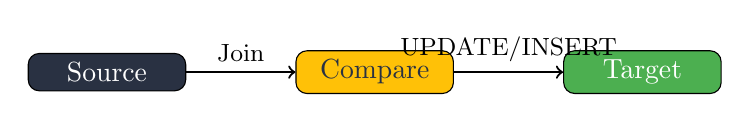
\begin{tikzpicture}[scale=0.85]
            \node[draw, fill=databricksBlue, text=white, rounded corners, minimum width=2cm] (source) at (0,0) {Source};
            \node[draw, fill=databricksYellow, text=databricksBlue, rounded corners, minimum width=2cm] (compare) at (4,0) {Compare};
            \node[draw, fill=databricksGreen, text=white, rounded corners, minimum width=2cm] (target) at (8,0) {Target};
            \draw[->, thick] (source) -- node[above, font=\small] {Join} (compare);
            \draw[->, thick] (compare) -- node[above, font=\small] {UPDATE/INSERT} (target);
        \end{tikzpicture}
    \end{center}
\end{frame}

% ============================================
% MERGE Clause Types
% ============================================
\begin{frame}[fragile]{MERGE Clause Types}
    \begin{columns}[T]
        \begin{column}{0.48\textwidth}
            \textcolor{databricksBlue}{\textbf{WHEN MATCHED:}}\\
            \small{Update or delete matching rows}
            \begin{lstlisting}[style=sqlstyle]
-- Update matching rows
WHEN MATCHED THEN
    UPDATE SET target.col1 = source.col1

-- With condition
WHEN MATCHED AND source.is_deleted = true 
THEN DELETE
WHEN MATCHED AND source.is_deleted = false 
THEN UPDATE SET target.col1 = source.col1
            \end{lstlisting}
        \end{column}
        \begin{column}{0.48\textwidth}
            \textcolor{databricksBlue}{\textbf{WHEN NOT MATCHED:}}\\
            \small{Insert new rows}
            \begin{lstlisting}[style=sqlstyle]
-- Insert new rows
WHEN NOT MATCHED THEN
    INSERT (id, name, value)
    VALUES (source.id, source.name, 
            source.value)
            \end{lstlisting}
            
            \vspace{0.2cm}
            \textcolor{databricksBlue}{\textbf{WHEN NOT MATCHED BY SOURCE:}}\\
            \small{Handle orphaned records}
            \begin{lstlisting}[style=sqlstyle]
-- Delete orphaned records
WHEN NOT MATCHED BY SOURCE THEN
    DELETE
            \end{lstlisting}
        \end{column}
    \end{columns}
\end{frame}

% ============================================
% MERGE with PySpark
% ============================================
\begin{frame}[fragile]{MERGE with PySpark}
    \begin{lstlisting}[style=pythonstyle]
from delta.tables import DeltaTable
from pyspark.sql.functions import current_timestamp

# Load the target Delta table
deltaTable = DeltaTable.forPath(spark, "/path/to/customers")

# Prepare source DataFrame
updates_df = spark.read.parquet("/path/to/updates")

# Perform MERGE
deltaTable.alias("target").merge(
    updates_df.alias("source"),
    "target.customer_id = source.customer_id"
).whenMatchedUpdate(
    condition="source.operation = 'UPDATE'",
    set={"name": "source.name", "email": "source.email",
         "modified_date": current_timestamp()}
).whenMatchedDelete(
    condition="source.operation = 'DELETE'"
).whenNotMatchedInsert(
    condition="source.operation = 'INSERT'",
    values={"customer_id": "source.customer_id", "name": "source.name",
            "created_date": current_timestamp()}
).execute()
    \end{lstlisting}
\end{frame}

% ============================================
% SECTION: OPTIMIZE & ZORDER
% ============================================
\begin{frame}[fragile]{The Small File Problem}
    \begin{columns}[T]
        \begin{column}{0.55\textwidth}
            \textcolor{databricksBlue}{\textbf{Why Small Files are Problematic:}}
            \vspace{0.3cm}
            \begin{itemize}
                \item \textcolor{databricksRed}{$\triangleright$} \textbf{Read Overhead}
                    \begin{itemize}
                        \item Each file requires metadata operations
                        \item 1000 × 1MB slower than 10 × 100MB
                    \end{itemize}
                \item \textcolor{databricksRed}{$\triangleright$} \textbf{Memory Pressure}
                    \begin{itemize}
                        \item Spark tracks all files in memory
                    \end{itemize}
                \item \textcolor{databricksRed}{$\triangleright$} \textbf{Cloud API Costs}
                    \begin{itemize}
                        \item More LIST and GET operations
                        \item Object stores charge per API call
                    \end{itemize}
            \end{itemize}
        \end{column}
        \begin{column}{0.42\textwidth}
            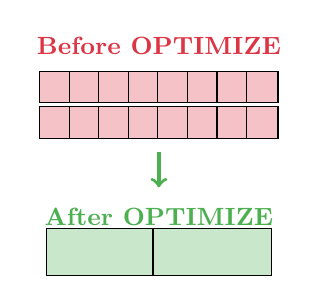
\begin{tikzpicture}[scale=0.75]
                % Small files (bad)
                \node[font=\small\bfseries, text=databricksRed] at (0,3.5) {Before OPTIMIZE};
                \foreach \i in {0,...,7} {
                    \node[draw, fill=databricksRed!30, minimum width=0.4cm, minimum height=0.4cm] at (\i*0.5-1.75,2.8) {};
                }
                \foreach \i in {0,...,7} {
                    \node[draw, fill=databricksRed!30, minimum width=0.4cm, minimum height=0.4cm] at (\i*0.5-1.75,2.2) {};
                }
                
                % Arrow
                \draw[->, very thick, databricksGreen] (0,1.7) -- (0,1.1);
                
                % Large files (good)
                \node[font=\small\bfseries, text=databricksGreen] at (0,0.6) {After OPTIMIZE};
                \node[draw, fill=databricksGreen!30, minimum width=1.5cm, minimum height=0.6cm] at (-0.9,0) {};
                \node[draw, fill=databricksGreen!30, minimum width=1.5cm, minimum height=0.6cm] at (0.9,0) {};
            \end{tikzpicture}
        \end{column}
    \end{columns}
\end{frame}

% ============================================
% OPTIMIZE Operation
% ============================================
\begin{frame}[fragile]{OPTIMIZE Operation}
    \textcolor{databricksBlue}{\textbf{Compacts small files into larger ones (target: ~1GB)}}
    
    \vspace{0.3cm}
    \begin{columns}[T]
        \begin{column}{0.48\textwidth}
            \textcolor{databricksBlue}{\textbf{SQL Syntax:}}
            \begin{lstlisting}[style=sqlstyle]
-- Basic OPTIMIZE
OPTIMIZE my_table;

-- Specific partitions
OPTIMIZE my_table 
WHERE date >= '2024-01-01';
            \end{lstlisting}
            
            \vspace{0.3cm}
            \textcolor{databricksBlue}{\textbf{PySpark:}}
            \begin{lstlisting}[style=pythonstyle]
from delta.tables import DeltaTable
deltaTable = DeltaTable.forPath(
    spark, "/path/to/table")
deltaTable.optimize()
    .executeCompaction()
            \end{lstlisting}
        \end{column}
        \begin{column}{0.48\textwidth}
            \textcolor{databricksBlue}{\textbf{How OPTIMIZE Works:}}
            \begin{enumerate}
                \item Identifies small files
                \item Groups files (respects partitions)
                \item Reads and rewrites data
                \item Updates transaction log atomically
                \item Original files marked for deletion
            \end{enumerate}
            
            \vspace{0.3cm}
            \textcolor{databricksRed}{\textbf{Note:}} Original files removed by VACUUM
        \end{column}
    \end{columns}
\end{frame}

% ============================================
% ZORDER Optimization
% ============================================
\begin{frame}[fragile]{ZORDER Optimization}
    \textcolor{databricksBlue}{\textbf{Co-locates related data in the same files for better data skipping}}
    
    \vspace{0.3cm}
    \begin{columns}[T]
        \begin{column}{0.48\textwidth}
            \begin{lstlisting}[style=sqlstyle]
-- ZORDER on specific columns
OPTIMIZE my_table 
ZORDER BY (customer_id);

-- Multiple columns
OPTIMIZE my_table 
ZORDER BY (region, customer_id);

-- Combined with partition filter
OPTIMIZE my_table 
WHERE date >= '2024-01-01' 
ZORDER BY (customer_id, product_id);
            \end{lstlisting}
        \end{column}
        \begin{column}{0.48\textwidth}
            \textcolor{databricksBlue}{\textbf{Good ZORDER Candidates:}}
            \begin{itemize}
                \item \textcolor{databricksGreen}{\faCheck} High-cardinality filter columns
                \item \textcolor{databricksGreen}{\faCheck} Columns used in JOINs
                \item \textcolor{databricksGreen}{\faCheck} WHERE clause columns
            \end{itemize}
            
            \vspace{0.3cm}
            \textcolor{databricksBlue}{\textbf{Poor Candidates:}}
            \begin{itemize}
                \item \textcolor{databricksRed}{\faTimes} Low-cardinality (use partition)
                \item \textcolor{databricksRed}{\faTimes} Rarely queried columns
                \item \textcolor{databricksRed}{\faTimes} Already partitioned columns
            \end{itemize}
        \end{column}
    \end{columns}
\end{frame}

% ============================================
% Partitioning vs ZORDER
% ============================================
\begin{frame}[fragile]{Partitioning vs ZORDER}
    \begin{center}
        \begin{tabular}{>{\raggedright}p{3.5cm}|>{\centering}p{4cm}|>{\centering\arraybackslash}p{4cm}}
            \toprule
            \rowcolor{databricksBlue}\textcolor{white}{\textbf{Characteristic}} & \textcolor{white}{\textbf{Use Partitioning}} & \textcolor{white}{\textbf{Use ZORDER}} \\
            \midrule
            Low cardinality (<1000) & \textcolor{databricksGreen}{\faCheck\ Yes} & \textcolor{databricksRed}{\faTimes\ No} \\
            \midrule
            High cardinality (>1000) & \textcolor{databricksRed}{\faTimes\ No} & \textcolor{databricksGreen}{\faCheck\ Yes} \\
            \midrule
            Used in every query & \textcolor{databricksGreen}{\faCheck\ Yes} & Less important \\
            \midrule
            Used in some queries & \textcolor{databricksRed}{\faTimes\ No} & \textcolor{databricksGreen}{\faCheck\ Yes} \\
            \midrule
            Equality predicates only & Yes (if low card) & Yes (if high card) \\
            \midrule
            Range predicates & \textcolor{databricksRed}{\faTimes\ No} & \textcolor{databricksGreen}{\faCheck\ Yes} \\
            \bottomrule
        \end{tabular}
    \end{center}
    
    \vspace{0.3cm}
    \textcolor{databricksBlue}{\textbf{Column Order Matters:}} First column has strongest locality
    \begin{lstlisting}[style=sqlstyle]
-- If most queries filter by customer_id first:
OPTIMIZE sales ZORDER BY (customer_id, product_id);
    \end{lstlisting}
\end{frame}

% ============================================
% Auto Optimize Features
% ============================================
\begin{frame}[fragile]{Auto Optimize Features}
    \begin{columns}[T]
        \begin{column}{0.48\textwidth}
            \textcolor{databricksBlue}{\textbf{Auto Compaction:}}\\
            \small{Automatically runs OPTIMIZE after writes}
            \begin{lstlisting}[style=sqlstyle]
-- Enable at table level
ALTER TABLE my_table SET TBLPROPERTIES (
  'delta.autoOptimize.autoCompact' 
    = 'true');

-- Enable for all tables in session
SET spark.databricks.delta
  .autoCompact.enabled = true;
            \end{lstlisting}
        \end{column}
        \begin{column}{0.48\textwidth}
            \textcolor{databricksBlue}{\textbf{Optimized Writes:}}\\
            \small{Coalesces small files during writes}
            \begin{lstlisting}[style=sqlstyle]
ALTER TABLE my_table SET TBLPROPERTIES (
  'delta.autoOptimize.optimizeWrite' 
    = 'true');
            \end{lstlisting}
            
            \vspace{0.3cm}
            \begin{tabular}{ll}
                \rowcolor{databricksLightGray}\textbf{Feature} & \textbf{When to Use} \\
                autoCompact & Streaming \\
                optimizeWrite & Frequent writes \\
                Manual & Batch maintenance \\
            \end{tabular}
        \end{column}
    \end{columns}
\end{frame}

% ============================================
% SECTION: VACUUM
% ============================================
\begin{frame}[fragile]{VACUUM for Cleanup}
    \textcolor{databricksBlue}{\textbf{Removes data files no longer referenced by the transaction log}}
    
    \vspace{0.3cm}
    \begin{columns}[T]
        \begin{column}{0.48\textwidth}
            \textcolor{databricksBlue}{\textbf{Why Files Become Stale:}}
            \begin{enumerate}
                \item New file written with updates
                \item Old file marked as ``removed''
                \item Old file still exists (for time travel)
                \item \textbf{VACUUM cleans them up}
            \end{enumerate}
            
            \vspace{0.3cm}
            \textcolor{databricksBlue}{\textbf{SQL Syntax:}}
            \begin{lstlisting}[style=sqlstyle]
-- Default 7-day retention
VACUUM my_table;

-- Custom retention
VACUUM my_table RETAIN 168 HOURS;

-- Dry run first!
VACUUM my_table DRY RUN;
            \end{lstlisting}
        \end{column}
        \begin{column}{0.48\textwidth}
            \textcolor{databricksBlue}{\textbf{PySpark:}}
            \begin{lstlisting}[style=pythonstyle]
from delta.tables import DeltaTable

deltaTable = DeltaTable.forPath(
    spark, "/path/to/table")

# Default retention
deltaTable.vacuum()

# Custom retention (hours)
deltaTable.vacuum(168)
            \end{lstlisting}
            
            \vspace{0.3cm}
            \textcolor{databricksRed}{\textbf{Warning:}} VACUUM affects time travel!
        \end{column}
    \end{columns}
\end{frame}

% ============================================
% VACUUM Retention & Safety
% ============================================
\begin{frame}[fragile]{VACUUM Retention \& Safety}
    \textcolor{databricksBlue}{\textbf{Recommended Retention Periods:}}
    
    \vspace{0.3cm}
    \begin{center}
        \begin{tabular}{>{\raggedright}p{4cm}|c|>{\raggedright\arraybackslash}p{5cm}}
            \toprule
            \rowcolor{databricksBlue}\textcolor{white}{\textbf{Scenario}} & \textcolor{white}{\textbf{Retention}} & \textcolor{white}{\textbf{Reasoning}} \\
            \midrule
            Production tables & 7-30 days & Balance cost \& recovery \\
            \midrule
            Development tables & 1-7 days & Lower cost, less recovery \\
            \midrule
            Audit-required tables & 30-365 days & Compliance requirements \\
            \midrule
            High-frequency updates & 7 days min & Protect long queries \\
            \bottomrule
        \end{tabular}
    \end{center}
    
    \vspace{0.3cm}
    \textcolor{databricksBlue}{\textbf{Align VACUUM with Time Travel:}}
    \begin{lstlisting}[style=sqlstyle]
-- If you need 30 days of time travel
ALTER TABLE my_table SET TBLPROPERTIES (
  'delta.logRetentionDuration' = '30 days',
  'delta.deletedFileRetentionDuration' = '30 days');

-- Then VACUUM with matching retention
VACUUM my_table RETAIN 720 HOURS;  -- 30 days
    \end{lstlisting}
\end{frame}

% ============================================
% OPTIMIZE vs VACUUM
% ============================================
\begin{frame}[fragile]{OPTIMIZE vs VACUUM Comparison}
    \begin{center}
        \begin{tabular}{>{\raggedright}p{3.5cm}|>{\centering}p{4cm}|>{\centering\arraybackslash}p{4cm}}
            \toprule
            \rowcolor{databricksBlue}\textcolor{white}{\textbf{Aspect}} & \textcolor{white}{\textbf{OPTIMIZE}} & \textcolor{white}{\textbf{VACUUM}} \\
            \midrule
            \textbf{Purpose} & Improve query performance & Reduce storage usage \\
            \midrule
            \textbf{Creates new files} & \textcolor{databricksGreen}{\faCheck\ Yes} & \textcolor{databricksRed}{\faTimes\ No} \\
            \midrule
            \textbf{Deletes files} & \textcolor{databricksRed}{\faTimes\ No} (marks stale) & \textcolor{databricksGreen}{\faCheck\ Yes} \\
            \midrule
            \textbf{Affects time travel} & \textcolor{databricksRed}{\faTimes\ No} & \textcolor{databricksGreen}{\faCheck\ Yes} \\
            \midrule
            \textbf{Storage impact} & Temporary increase & Decrease \\
            \midrule
            \textbf{When to run} & After many writes & After OPTIMIZE \\
            \midrule
            \textbf{Frequency} & Daily or weekly & Weekly or monthly \\
            \bottomrule
        \end{tabular}
    \end{center}
    
    \vspace{0.3cm}
    \textcolor{databricksBlue}{\textbf{Typical Workflow:}} Write Data → OPTIMIZE → VACUUM
\end{frame}

% ============================================
% Best Practices
% ============================================
\begin{frame}[fragile]{Best Practices \& Performance Tips}
    \begin{columns}[T]
        \begin{column}{0.48\textwidth}
            \textcolor{databricksBlue}{\textbf{Table Design:}}
            \begin{itemize}
                \item \textcolor{databricksRed}{$\triangleright$} Partition by low-cardinality columns
                \item \textcolor{databricksRed}{$\triangleright$} Aim for 1GB+ partitions
                \item \textcolor{databricksRed}{$\triangleright$} Avoid >10,000 partitions
                \item \textcolor{databricksRed}{$\triangleright$} ZORDER high-cardinality columns
            \end{itemize}
            
            \vspace{0.3cm}
            \textcolor{databricksBlue}{\textbf{MERGE Optimization:}}
            \begin{itemize}
                \item \textcolor{databricksRed}{$\triangleright$} Pre-filter source data
                \item \textcolor{databricksRed}{$\triangleright$} Include partition columns in join
                \item \textcolor{databricksRed}{$\triangleright$} Batch small merges
            \end{itemize}
        \end{column}
        \begin{column}{0.48\textwidth}
            \textcolor{databricksBlue}{\textbf{OPTIMIZE Schedule:}}
            \begin{itemize}
                \item \textcolor{databricksRed}{$\triangleright$} Streaming: Every 1-4 hours
                \item \textcolor{databricksRed}{$\triangleright$} Micro-batch: Daily
                \item \textcolor{databricksRed}{$\triangleright$} Batch: After each load
            \end{itemize}
            
            \vspace{0.3cm}
            \textcolor{databricksBlue}{\textbf{VACUUM Guidelines:}}
            \begin{itemize}
                \item \textcolor{databricksRed}{$\triangleright$} Never <7 days without understanding
                \item \textcolor{databricksRed}{$\triangleright$} Always DRY RUN first
                \item \textcolor{databricksRed}{$\triangleright$} Run during low-traffic periods
                \item \textcolor{databricksRed}{$\triangleright$} Schedule after OPTIMIZE
            \end{itemize}
        \end{column}
    \end{columns}
\end{frame}

% ============================================
% Common Pitfalls
% ============================================
\begin{frame}[fragile]{Common Pitfalls to Avoid}
    \begin{center}
        \begin{tabular}{>{\raggedright}p{3cm}|>{\raggedright}p{4cm}|>{\raggedright\arraybackslash}p{4.5cm}}
            \toprule
            \rowcolor{databricksBlue}\textcolor{white}{\textbf{Pitfall}} & \textcolor{white}{\textbf{Problem}} & \textcolor{white}{\textbf{Solution}} \\
            \midrule
            Over-partitioning & Too many small files & Fewer partitions, use ZORDER \\
            \midrule
            ZORDER on partition cols & Redundant, no benefit & ZORDER non-partition columns \\
            \midrule
            Aggressive VACUUM & Lose time travel & Match retention to needs \\
            \midrule
            No OPTIMIZE schedule & Small file problem & Automate with Auto Optimize \\
            \midrule
            MERGE without filters & Full table rewrite & Pre-filter, partition pruning \\
            \midrule
            Ignoring file stats & Poor data skipping & ZORDER filtered columns \\
            \bottomrule
        \end{tabular}
    \end{center}
\end{frame}

% ============================================
% Quick Reference Card
% ============================================
\begin{frame}[fragile]{Quick Reference Card}
    \begin{columns}[T]
        \begin{column}{0.48\textwidth}
            \textcolor{databricksBlue}{\textbf{Time Travel Commands:}}
            \begin{lstlisting}[style=sqlstyle]
SELECT * FROM t VERSION AS OF 5;
SELECT * FROM t TIMESTAMP AS OF 
  '2024-01-15';
DESCRIBE HISTORY t;
RESTORE TABLE t TO VERSION AS OF 5;
            \end{lstlisting}
            
            \vspace{0.3cm}
            \textcolor{databricksBlue}{\textbf{MERGE Pattern:}}
            \begin{lstlisting}[style=sqlstyle]
MERGE INTO target USING source 
ON condition
WHEN MATCHED THEN UPDATE SET ...
WHEN NOT MATCHED THEN INSERT ...
            \end{lstlisting}
        \end{column}
        \begin{column}{0.48\textwidth}
            \textcolor{databricksBlue}{\textbf{OPTIMIZE \& VACUUM:}}
            \begin{lstlisting}[style=sqlstyle]
OPTIMIZE t;
OPTIMIZE t ZORDER BY (col1, col2);
OPTIMIZE t WHERE partition_col = 'v';
VACUUM t;
VACUUM t RETAIN 168 HOURS;
VACUUM t DRY RUN;
            \end{lstlisting}
            
            \vspace{0.3cm}
            \textcolor{databricksBlue}{\textbf{Key Properties:}}
            \begin{lstlisting}[style=sqlstyle]
'delta.logRetentionDuration'
'delta.deletedFileRetentionDuration'
'delta.autoOptimize.optimizeWrite'
'delta.autoOptimize.autoCompact'
            \end{lstlisting}
        \end{column}
    \end{columns}
\end{frame}

% ============================================
% THANK YOU SLIDE
% ============================================
\begin{frame}[plain]
    \begin{tikzpicture}[remember picture,overlay]
        \fill[databricksBlue] (current page.north west) rectangle (current page.south east);
    \end{tikzpicture}
    \vfill
    \begin{center}
        {\Huge\textcolor{databricksWhite}{\textbf{Thank You!}}\par}
        \vspace{0.8cm}
        {\Large\textcolor{databricksYellow}{Questions?}\par}
        \vspace{1.5cm}
        {\large\textcolor{databricksWhite}{
            \faLinkedin\ \href{https://www.linkedin.com/in/yashkavaiya}{linkedin.com/in/yashkavaiya}
        }\par}
        \vspace{0.3cm}
        {\large\textcolor{databricksWhite}{
            \faRocket\ \href{https://easy-ai-labs.lovable.app/}{easy-ai-labs.lovable.app}
        }\par}
        \vspace{0.3cm}
        {\large\textcolor{databricksWhite}{
            \faUsers\ \href{https://www.linkedin.com/company/genai-guru}{Gen AI Guru}
        }\par}
    \end{center}
    \vfill
\end{frame}

\end{document}


